\documentclass[11pt,a4paper]{article}
\usepackage[margin=2.5cm]{geometry}
\usepackage{amsmath,amssymb}
\usepackage{graphicx}
\usepackage{listings}
\usepackage{xcolor}
\usepackage{hyperref}
\usepackage{booktabs}
\usepackage{tikz}
\usetikzlibrary{arrows.meta,positioning,shapes.geometric}

\hypersetup{colorlinks=true, linkcolor=blue, urlcolor=blue}

\lstset{
  language=Python,
  basicstyle=\ttfamily\small,
  keywordstyle=\color{blue}\bfseries,
  commentstyle=\color{gray},
  stringstyle=\color{teal},
  numbers=left, numberstyle=\tiny\color{gray},
  frame=single, breaklines=true,
  backgroundcolor=\color{gray!5}
}

\title{\textbf{From Simulation to Over-the-Air:\\
OFDM with PlutoSDR}\\\large Experiment 04 --- IIT Dharwad}
\author{Dept.\ of EECE, IIT Dharwad}
\date{}

\begin{document}
\maketitle
\tableofcontents
\bigskip

% ─────────────────────────────────────────────────────────────────────────────
\section{Motivation: What Changes When You Go Over-the-Air?}

In simulation you handed a complex baseband array directly from transmitter to
receiver, possibly adding white noise.  The real channel introduces several
impairments that a simulation loop typically ignores:

\begin{center}
\begin{tabular}{p{4cm}p{5.5cm}p{4.5cm}}
\toprule
\textbf{Impairment} & \textbf{Cause} & \textbf{Fix needed} \\
\midrule
Unknown frame start & propagation delay + async clocks & Timing synchronisation \\
Carrier freq.\ offset (CFO) & TX/RX oscillators differ by $\Delta f$ & CFO estimation + correction \\
Multipath fading & signal arrives via multiple paths & Channel estimation + equalisation \\
Noise & thermal, quantisation & handled by modulation SNR margin \\
DC offset & LO leakage in direct-conversion radio & DC removal \\
Amplitude variation & distance, antenna gain & AGC \\
\bottomrule
\end{tabular}
\end{center}

This writeup explains \emph{every} block added to the RX chain beyond what you
already know from simulation.

% ─────────────────────────────────────────────────────────────────────────────
\section{System Overview}

\subsection{Frame Structure}

The transmitter sends a cyclic stream of identical frames:

\begin{center}
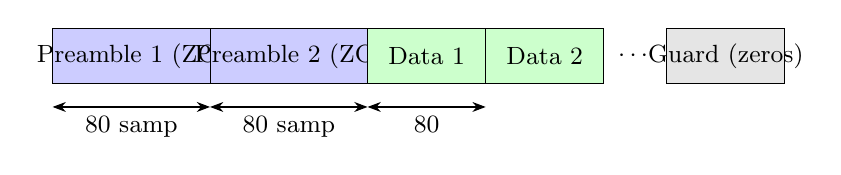
\begin{tikzpicture}[every node/.style={font=\small}, >=Stealth]
  \def\h{0.7}
  \draw[fill=blue!20]  (0,0)   rectangle (2,\h) node[midway]{Preamble 1 (ZC)};
  \draw[fill=blue!20]  (2,0)   rectangle (4,\h) node[midway]{Preamble 2 (ZC)};
  \draw[fill=green!20] (4,0)   rectangle (5.5,\h) node[midway]{Data 1};
  \draw[fill=green!20] (5.5,0) rectangle (7,\h)   node[midway]{Data 2};
  \node at (7.4,\h/2) {$\cdots$};
  \draw[fill=gray!20]  (7.8,0) rectangle (9.3,\h) node[midway]{Guard (zeros)};
  \draw[<->] (0,-0.3) -- (2,-0.3) node[midway,below]{80 samp};
  \draw[<->] (2,-0.3) -- (4,-0.3) node[midway,below]{80 samp};
  \draw[<->] (4,-0.3) -- (5.5,-0.3) node[midway,below]{80};
\end{tikzpicture}
\end{center}

Each symbol is 80 samples: 16-sample cyclic prefix (CP) + 64-sample IFFT output.
The two identical preamble symbols each serve a specific role:
\begin{itemize}
  \item \textbf{Timing}: both preambles together (paired-peak detector, \S\ref{sec:timing})
  \item \textbf{CFO estimation}: phase difference between the two FFTs (\S3)
  \item \textbf{Channel estimation}: preamble-1 FFT only (\S5)
\end{itemize}

\subsection{Subcarrier Map (64-point FFT)}

Each FFT bin spans $F_s/N = 2\,\text{MHz}/64 = 31.25\,\text{kHz}$.

\begin{center}
\begin{tabular}{p{3.5cm}p{3cm}cp{5cm}}
\toprule
\textbf{Subcarriers} & \textbf{Indices} & \textbf{Count} & \textbf{Reason nulled} \\
\midrule
DC & 0 & 1 & LO leakage in direct-conversion radio appears at DC; always nulled \\
Guard band & 27--37 & 11 &
  These straddle the Nyquist point (bin~32 $= F_s/2 = 1\,\text{MHz}$).
  Nulling them gives the anti-alias filter room to roll off without
  corrupting edge subcarriers. \\
\midrule
Data & 1--26, 38--63 minus pilots & 48 & Carry payload bits \\
Pilots & 7, 21, 43, 57 & 4 &
  Transmitted with known ZC values; \emph{not used by the current RX}
  (see note below). \\
\midrule
Active (data + pilots) & & 52 & \\
\bottomrule
\end{tabular}
\end{center}

\paragraph{Note on pilots.}
The TX inserts known ZC values on the 4 pilot subcarriers of \emph{every data
symbol}.  In a production receiver these would be used to \emph{track}
phase and amplitude drift on a symbol-by-symbol basis (phase-locked loop
per subcarrier, or least-squares update each symbol).  The current RX
does \textbf{not} use them: it applies the single preamble-based channel
estimate $\hat{H}[k]$ to all data symbols unchanged.  This is sufficient
when the channel is stable over the frame duration (which it is for a
static indoor link).  A natural extension is to update $\hat{H}[k]$ each
symbol using the pilot subcarriers --- see Exercise~6.

\subsection{RX Pipeline}

\begin{center}
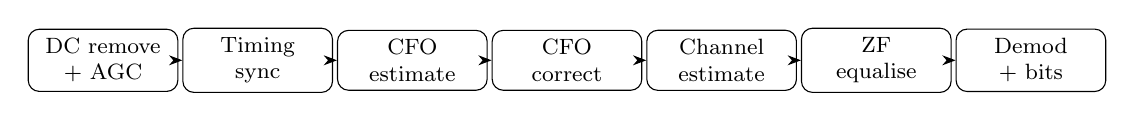
\begin{tikzpicture}[node distance=0.4cm and 0.05cm, every node/.style={font=\footnotesize},
    box/.style={draw, rounded corners, fill=white, minimum width=1.9cm,
                minimum height=0.6cm, align=center},
    >=Stealth]
  \node[box] (dc)  {DC remove\\+ AGC};
  \node[box, right=of dc]  (tim) {Timing\\sync};
  \node[box, right=of tim] (cfo) {CFO\\estimate};
  \node[box, right=of cfo] (cor) {CFO\\correct};
  \node[box, right=of cor] (che) {Channel\\estimate};
  \node[box, right=of che] (eq)  {ZF\\equalise};
  \node[box, right=of eq]  (dem) {Demod\\+ bits};
  \draw[->] (dc)--(tim); \draw[->] (tim)--(cfo); \draw[->] (cfo)--(cor);
  \draw[->] (cor)--(che); \draw[->] (che)--(eq); \draw[->] (eq)--(dem);
\end{tikzpicture}
\end{center}

% ─────────────────────────────────────────────────────────────────────────────
\section{The Zadoff-Chu Preamble}

\subsection{Definition}

A Zadoff-Chu (ZC) sequence of length $N_u$ with root $q$ is:
\begin{equation}
  x[n] = \exp\!\left(-j\pi q\,\frac{n(n+1)}{N_u}\right), \quad n = 0,1,\ldots,N_u-1
\end{equation}

Here $N_u = 52$ (number of active subcarriers), $q = 1$.

\subsection{Why ZC?}

\begin{enumerate}
  \item \textbf{Constant amplitude (CAZAC)}: $|x[n]| = 1$ for all $n$ ---
        the sequence has \emph{Constant Amplitude Zero AutoCorrelation}.
        No subcarrier carries more power than any other.
  \item \textbf{Perfect periodic autocorrelation}: $|R_{xx}[\tau]| = 0$ for
        $\tau \neq 0 \pmod{N_u}$, so the cross-correlation with the reference
        produces a single sharp spike.  This gives unambiguous, sample-accurate
        timing.
  \item \textbf{Flat magnitude spectrum}: placing ZC values on all 52 active
        subcarriers gives a nearly uniform power spectral density, which means
        every active subcarrier contributes equally to channel estimation ---
        no subcarrier is better illuminated than another.
  \item \textbf{Known to both sides}: the RX stores the reference time-domain
        signal $\mathbf{p}$ computed from the same formula; no side channel
        needed.
\end{enumerate}

\subsection{Implementation}

\begin{lstlisting}
def _zc(length, order=1):
    n = np.arange(length)
    return np.exp(-1j * np.pi * order * n * (n + 1) / length)

ZC_ACTIVE = _zc(52)          # 52-point ZC on active subcarriers

# Build preamble OFDM symbol (with CP)
fd = np.zeros(64, dtype=complex)
fd[ACTIVE_IDX] = ZC_ACTIVE   # place ZC on 52 active subs; rest = 0
td = np.fft.ifft(fd) * np.sqrt(64)
preamble = np.concatenate([td[-16:], td])   # prepend CP
\end{lstlisting}

The preamble symbol therefore looks like a normal OFDM symbol except every
active subcarrier carries a known ZC value.

% ─────────────────────────────────────────────────────────────────────────────
\section{Block 1: DC Removal and AGC}

\textbf{DC removal} subtracts the sample mean.
LO leakage in a direct-conversion receiver like Pluto injects a constant
(DC) tone at bin~0; if left uncorrected it desensitises the correlator.

\textbf{AGC} (automatic gain control) normalises the buffer energy to 1:
\begin{equation}
  \hat{x}[n] = \frac{x[n]}{\sqrt{\frac{1}{N}\sum_k |x[k]|^2}}
\end{equation}
This makes the normalised correlation threshold (\S\ref{sec:timing}) a
fixed, signal-level-independent constant.

% ─────────────────────────────────────────────────────────────────────────────
\section{Block 2: Timing Synchronisation}
\label{sec:timing}

\subsection{Goal}

Find the sample index where the first preamble symbol \emph{(excluding its CP)}
starts in the received buffer.

\subsection{Normalised Cross-Correlation}

The raw correlation between the received signal and the reference preamble
$\mathbf{p}$ (64 samples, no CP) is:
\begin{equation}
  C[n] = \left|\sum_{k=0}^{63} r[n+k]\, p^*[k]\right|
\end{equation}

To make the threshold independent of received power, normalise by the local
energy of the received signal:
\begin{equation}
  \hat{C}[n] = \frac{C[n]}{\sqrt{E_{\text{local}}[n] \cdot E_p}}, \qquad
  E_{\text{local}}[n] = \sum_{k=0}^{63}|r[n+k]|^2
\end{equation}

$\hat{C}[n] \in [0,1]$ with $\hat{C}[n]=1$ at a perfect noiseless match.

\subsection{The Paired-Peak Problem}

The TX sends \emph{two identical} preamble symbols.  A simple $\arg\max
\hat{C}$ would sometimes lock onto preamble~2 (at position
$n^* + 80$) instead of preamble~1 (at $n^*$) because both produce equally
strong peaks.  This shifts every downstream index by 80 samples, corrupting
the decode.

\subsection{Paired-Peak Detector}

The solution: require two peaks separated by exactly $T_s = 80$ samples.
Define the \emph{paired metric}:
\begin{equation}
  \text{paired}[n] = \hat{C}[n] + \hat{C}[n + 80]
\end{equation}
and take
\begin{equation}
  \hat{n} = \arg\max_n\, \text{paired}[n]
\end{equation}

$\hat{n}$ is unambiguously the start of preamble~1 because only that position
gives a \emph{simultaneous} high-correlation match at both $\hat{n}$ and
$\hat{n}+80$.  The threshold is applied to
$\text{score} = \text{paired}[\hat{n}]/2$.

\begin{lstlisting}
# Reference: preamble without CP, 64 samples
_td_ref   = (np.fft.ifft(_fd_ref) * np.sqrt(64)).astype(np.complex64)
_REF_PWR  = float(np.dot(_td_ref, _td_ref.conj()).real)

corr      = np.abs(correlate(rx, _td_ref, mode='valid'))
local_e   = np.convolve(np.abs(rx)**2, np.ones(64), mode='valid') + 1e-10
norm_corr = corr / np.sqrt(local_e * _REF_PWR)

paired    = norm_corr[:-80] + norm_corr[80:]
best      = int(np.argmax(paired))
score     = float(paired[best]) / 2
if score < 0.50:
    return None, score          # no frame found
return best, score              # best = no-CP start of preamble-1
\end{lstlisting}

A threshold of 0.50 works well in practice: noise alone scores $\sim0.33$,
a clean ZC preamble at 20\,dB SNR scores $>0.90$.

% ─────────────────────────────────────────────────────────────────────────────
\section{Block 3: CFO Estimation}

\subsection{Problem}

The TX Pluto and RX Pluto have independent 40\,MHz TCXO references.
Even a $1\,\text{ppm}$ error at 915\,MHz gives $\Delta f = 915\,\text{Hz}$.
A CFO of $\Delta f$ multiplies the received signal by $e^{j2\pi\Delta f t}$,
which in the frequency domain shifts every subcarrier by a non-integer amount,
causing \emph{inter-carrier interference (ICI)}.

\subsection{Two-Preamble Phase Estimator}

Both preamble symbols carry the identical ZC sequence.  After propagating
through the same channel $H[k]$, the received frequency-domain preambles are:
\begin{align}
  P_1[k] &= H[k]\,X_{\text{ZC}}[k]\cdot e^{j\phi_1[k]} \\
  P_2[k] &= H[k]\,X_{\text{ZC}}[k]\cdot e^{j\phi_2[k]}
\end{align}
where the phase difference accumulated over one symbol period $T_s = 80/F_s$
is:
\begin{equation}
  \phi_2[k] - \phi_1[k] = 2\pi\,\Delta f\, T_s
\end{equation}

Taking the conjugate product and averaging over all 52 active subcarriers
cancels the channel and noise:
\begin{equation}
  \angle\!\left(\frac{1}{52}\sum_{k \in \mathcal{A}} P_2[k]\,P_1^*[k]\right)
  = 2\pi\,\Delta f\, T_s
\end{equation}

Solving for $\Delta f$:
\begin{equation}
  \boxed{\hat{\Delta f} = \frac{F_s}{2\pi\,T_s}\,
    \angle\!\left(\frac{1}{52}\sum_{k \in \mathcal{A}} P_2[k]\,P_1^*[k]\right)}
\end{equation}

\textbf{Unambiguous range}: $|\Delta f| < F_s/(2T_s) = 12.5\,\text{kHz}$ at
2\,MSPS --- far larger than any Pluto-to-Pluto mismatch.

\begin{lstlisting}
P1 = np.fft.fft(rx[ps        : ps+64])    / np.sqrt(64)
P2 = np.fft.fft(rx[ps+80     : ps+80+64]) / np.sqrt(64)

delta = P2[ACTIVE_IDX] * np.conj(P1[ACTIVE_IDX])
phase = np.angle(np.mean(delta))
cfo_hz = phase * fs / (2 * np.pi * 80)
\end{lstlisting}

% ─────────────────────────────────────────────────────────────────────────────
\section{Block 4: CFO Correction}

Once $\hat{\Delta f}$ is known, multiply the entire receive buffer by a
counter-rotating phasor:
\begin{equation}
  r_c[n] = r[n]\cdot e^{-j2\pi\hat{\Delta f}\,n/F_s}
\end{equation}

\begin{lstlisting}
t      = np.arange(len(rx)) / fs
rx_cfo = rx * np.exp(-1j * 2 * np.pi * cfo_hz * t)
\end{lstlisting}

After correction, timing is re-run on $r_c$ to pick up any small positional
shift introduced by the phase ramp.

% ─────────────────────────────────────────────────────────────────────────────
\section{Block 5: Channel Estimation}

\subsection{Least-Squares (LS) Estimate on the Preamble}

The received frequency-domain preamble-1 (after FFT, no CP) is:
\begin{equation}
  Y_p[k] = H[k]\,X_{\text{ZC}}[k] + W[k], \quad k \in \mathcal{A}
\end{equation}

Since both $Y_p[k]$ and $X_{\text{ZC}}[k]$ are known at the receiver, the LS
channel estimate at each active subcarrier is simply a division:
\begin{equation}
  \hat{H}[k] = \frac{Y_p[k]}{X_{\text{ZC}}[k]}, \quad k \in \mathcal{A}
\end{equation}

This gives 52 complex channel samples (amplitude + phase) at the active
subcarrier positions.

\subsection{Interpolation to All 64 Subcarriers}

Data subcarriers need a channel estimate too, but the preamble only populates
the 52 active positions.  Linear interpolation fills in the rest:
\begin{equation}
  \hat{H}[k] = \text{interp}\!\left(k;\;
    \{k_i, \hat{H}[k_i]\}_{k_i \in \mathcal{A}}\right), \quad k = 0,\ldots,63
\end{equation}
Real and imaginary parts are interpolated independently.

\begin{lstlisting}
p1_fd   = np.fft.fft(rx_cfo[ps : ps+64]) / np.sqrt(64)
H_active = p1_fd[ACTIVE_IDX] / ZC_ACTIVE      # LS: 52 values

H_all = (np.interp(np.arange(64), ACTIVE_IDX, np.real(H_active)) +
     1j * np.interp(np.arange(64), ACTIVE_IDX, np.imag(H_active)))
\end{lstlisting}

\subsection{Why Use the Preamble, Not Pilots?}

The preamble gives 52 channel samples across the band in one shot, before any
data arrives, at no additional throughput cost.  The 4 pilot subcarriers per
data symbol would give a much coarser 4-point estimate.  For a short burst over
a static channel, the single preamble estimate is sufficient.

% ─────────────────────────────────────────────────────────────────────────────
\section{Block 6: Zero-Forcing Equalisation}

For each data OFDM symbol, the received frequency-domain data at subcarrier $k$
is:
\begin{equation}
  Y_d[k] = H[k]\,S[k] + W[k]
\end{equation}
where $S[k]$ is the transmitted data symbol (unknown).

Zero-forcing inverts the channel estimate to recover $S[k]$:
\begin{equation}
  \hat{S}[k] = \frac{Y_d[k]}{\hat{H}[k]}
\end{equation}

The regularisation $\hat{H}[k] + \epsilon$ (with $\epsilon = 10^{-8}$) prevents
division by zero on deeply faded subcarriers.

\subsection{Data Symbol Index Arithmetic}

A common source of bugs is computing the correct sample index for each data
symbol.  The diagram below shows the layout:

\begin{center}
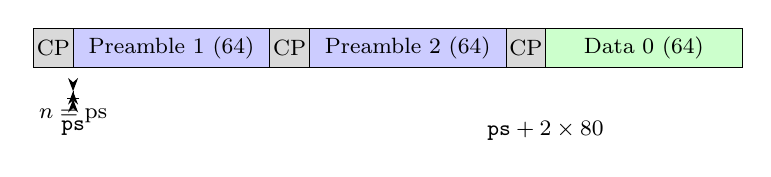
\begin{tikzpicture}[every node/.style={font=\footnotesize}, >=Stealth]
  \def\h{0.5}
  \draw[fill=gray!30] (0,0)  rectangle (0.5,\h) node[midway]{CP};
  \draw[fill=blue!20] (0.5,0) rectangle (3,\h)  node[midway]{Preamble 1 (64)};
  \draw[fill=gray!30] (3,0)  rectangle (3.5,\h) node[midway]{CP};
  \draw[fill=blue!20] (3.5,0) rectangle (6,\h)  node[midway]{Preamble 2 (64)};
  \draw[fill=gray!30] (6,0)  rectangle (6.5,\h) node[midway]{CP};
  \draw[fill=green!20](6.5,0) rectangle (9,\h)  node[midway]{Data 0 (64)};
  \draw[<->] (0.5,-0.3) -- (0.5,-0.3) ;
  \draw[|->] (0.5,-0.4) node[below]{$n = \text{ps}$} -- (0.5,-0.4);
  \node[below] at (0.5,-0.55) {$\mathtt{ps}$};
  \node[below] at (6.5,-0.55) {$\mathtt{ps} + 2\times80$};
\end{tikzpicture}
\end{center}

\texttt{ps} is the no-CP start of preamble~1.  Data symbol $i$ (no-CP) starts at:
\begin{equation}
  \label{eq:ds_start}
  n_i = \underbrace{\text{ps}}_{\text{pream-1 no-CP}}
        + \underbrace{2 \times 80}_{\text{2 preamble symbols}}
        + \underbrace{i \times 80}_{\text{i data symbols}}
\end{equation}

Note the CP of the data symbol is \emph{already included} in the $80i$ stride;
the 64-sample FFT window starts at $n_i$ (CP already skipped), which works
because the CP of each symbol is of length 16 and is absorbed into the stride.

\begin{lstlisting}
for i in range(n_data_syms):
    ds_start = ps + 2 * 80 + i * 80   # no-CP start of data symbol i
    ds_td    = rx_cfo[ds_start : ds_start + 64]
    ds_fd    = np.fft.fft(ds_td) / np.sqrt(64)
    ds_eq    = ds_fd / (H_all + 1e-8)
    bits     = symbols_to_bits(ds_eq[DATA_IDX], scheme)
\end{lstlisting}

% ─────────────────────────────────────────────────────────────────────────────
\section{Block 7: Demodulation}

After equalisation, \texttt{ds\_eq[DATA\_IDX]} is a 48-element complex array of
recovered QPSK (or QAM) symbols.  Hard-decision demodulation maps each point
to the nearest constellation point (in Gray code order) and extracts bits.
This is identical to the simulation version --- the channel and sync pipeline
has done all the work to present clean constellation points to this stage.

% ─────────────────────────────────────────────────────────────────────────────
\section{Preamble Quality Score}

The code reports a link quality metric derived from the preamble channel
estimate.  It is \textbf{not} standard EVM (which would require comparing
equalized data symbols to the ideal constellation).

\subsection{What the Code Computes}

After LS estimation, $\hat{H}[k]$ is the channel at each active subcarrier.
For a perfect flat channel with unit gain and zero phase, $\hat{H}[k] = 1$.
The code measures the deviation of the channel estimate at the 4 pilot
subcarrier positions from this ideal:
\begin{equation}
  Q = 10\log_{10}\!\left(\frac{1}{4}\sum_{p \in \text{pilots}}
    \left|\hat{H}[k_p] - 1\right|^2\right) \text{ dB}
\end{equation}

This is a \emph{channel quality score}: it is large (positive dB) when the
channel has significant gain variation or phase shift across the band, and
small (negative dB) only for a near-ideal flat channel.

\subsection{Why It Is Not Standard EVM}

Standard EVM compares the received equalized constellation point to the ideal
transmitted symbol:
\begin{equation}
  \text{EVM}_{\text{std}} = \sqrt{\frac{\sum_k |\hat{S}[k] - S[k]|^2}
    {\sum_k |S[k]|^2}}
\end{equation}
This requires knowing the transmitted symbols $S[k]$, which the RX does not
have without decision feedback or a known pilot sequence per data symbol.

\subsection{Interpreting the Reported Values}

\begin{center}
\begin{tabular}{ll}
\toprule
\textbf{Reported Q (dB)} & \textbf{Interpretation} \\
\midrule
$< 0$ & Channel is nearly flat and unit-gain at pilots \\
$0$--$10$ & Moderate channel variation; QPSK typically still works \\
$> 15$ & Significant channel non-flatness or phase offset; decode may degrade \\
\bottomrule
\end{tabular}
\end{center}

In the OTA test here, Q was $+11$ to $+15$\,dB, indicating a moderately
frequency-selective channel between the two Plutos.  BER was still 0 for QPSK
because the LS channel estimate correctly captured $\hat{H}[k]$ and the ZF
equaliser divided it out --- the magnitude of $\hat{H}[k]$ does not need to be 1
for decoding to succeed; it just needs to be estimated accurately.

% ─────────────────────────────────────────────────────────────────────────────
\section{Hardware Details: Cyclic TX Buffer}

Setting \texttt{sdr.tx\_cyclic\_buffer = True} tells the Pluto firmware to
loop the IQ buffer in hardware without any Python involvement.  This is
critical: Python's GC pauses would otherwise create gaps in the transmitted
waveform that break timing and channel estimation.

The IQ data must be scaled to the Pluto's 12-bit DAC range.  We keep 6\,dB
headroom for OFDM's inherent PAPR:
\begin{lstlisting}
peak = np.max(np.abs(frame)) + 1e-9
iq   = (frame * (2**13 / peak)).astype(np.complex64)
sdr.tx(iq)
\end{lstlisting}

% ─────────────────────────────────────────────────────────────────────────────
\section{Measured OTA Results}

\begin{lstlisting}[language={},basicstyle=\ttfamily\small]
[TX] Text    : "Hello IIT Dharwad! OFDM OTA test."
[TX] Scheme  : QPSK  |  Data syms: 3
[TX] FC=915.000 MHz  FS=2.0 MSPS  att=-30.0 dB

[RX] FC=915.000 MHz  FS=2.0 MSPS  scheme=QPSK  gain=50.0 dB

  [  1]  corr=0.93  CFO=-2696 Hz  syms=3  EVM=14.6 dB  "Hello IIT Dharwad! OFDM OTA test."
  [  2]  corr=0.95  CFO=-3060 Hz  syms=3  EVM=11.2 dB  "Hello IIT Dharwad! OFDM OTA test."
  [  3]  corr=0.95  CFO=-2823 Hz  syms=3  EVM=12.5 dB  "Hello IIT Dharwad! OFDM OTA test."
  [  4]  corr=0.93  CFO=-3049 Hz  syms=3  EVM=15.3 dB  "Hello IIT Dharwad! OFDM OTA test."
  [  5]  corr=0.96  CFO=-3074 Hz  syms=3  EVM=13.3 dB  "Hello IIT Dharwad! OFDM OTA test."

Decoded 5/5  |  Missed 0
\end{lstlisting}

The CFO of $\approx -3\,\text{kHz}$ at 915\,MHz corresponds to a crystal
mismatch of $\approx 3.3\,\text{ppm}$ between the two Plutos, well within
the $\pm 12.5\,\text{kHz}$ unambiguous range of the estimator.

% ─────────────────────────────────────────────────────────────────────────────
\section{Running the Code}

Open two terminals in \texttt{experiments/04\_ofdm/}:

\begin{lstlisting}[language=bash]
# Terminal 1 — transmitter
python ofdm_tx.py --text "Hello IIT Dharwad!" --scheme QPSK --att -30

# Terminal 2 — receiver (run while TX is cycling)
python ofdm_rx.py --scheme QPSK --n_frames 10 --max_syms 3
\end{lstlisting}

\textbf{Key arguments:}
\begin{itemize}
  \item \texttt{--scheme}: \texttt{BPSK} / \texttt{QPSK} / \texttt{QAM16}
  \item \texttt{--att}: TX attenuation in dB (0\,=\,max power; $-89$\,=\,min)
  \item \texttt{--max\_syms}: limit RX to the known data-symbol count; avoids decoding noise after the frame
  \item \texttt{--threshold}: preamble detection threshold (default 0.50; lower if corr $<$ 0.5 at low SNR)
  \item \texttt{--gain}: RX gain in dB (default 50)
\end{itemize}

\textbf{If the TX crashes with \texttt{OSError: [Errno 16] Device or resource busy}:}
a previous cyclic buffer was not released.  Run:
\begin{lstlisting}
python -c "
import sys; sys.path.insert(0,'../../')
from common.pluto_config import connect_tx
sdr = connect_tx(fc=915000000, fs=2000000, gain_att=-30)
sdr.tx_destroy_buffer()
print('released')
"
\end{lstlisting}

% ─────────────────────────────────────────────────────────────────────────────
\section{Exercises}

\begin{enumerate}
  \item \textbf{CFO stress test.}  Record the estimated CFO from 20 consecutive
    frames.  Does it stay stable?  What does drift imply about oscillator
    stability?

  \item \textbf{Modulation order.}  Change \texttt{--scheme} to \texttt{QAM16}.
    What happens to the EVM?  At what TX attenuation does BER increase?

  \item \textbf{Distance.}  Move the antennas further apart.  Plot EVM
    vs.\ distance.  Relate it to the free-space path loss formula
    $L = (4\pi d f / c)^2$.

  \item \textbf{Multipath.}  Place a metal reflector behind the RX antenna.
    Does the EVM change?  Why?  (Hint: the preamble-based channel estimate
    should adapt automatically.)

  \item \textbf{Threshold.}  Lower \texttt{--threshold} to 0.30 and observe
    false detections when the TX is switched off.  Restore to 0.50 and verify
    they disappear.  What is the noise floor score?

  \item \textbf{Add a length field.}  The current frame has no header telling
    the RX how many data symbols to decode.  Add a 1-byte header as the first
    data symbol so the RX can set \texttt{max\_syms} automatically.

  \item \textbf{Use pilots for per-symbol channel tracking.}
    Currently the 4 pilot subcarriers (indices 7, 21, 43, 57) are transmitted
    with known ZC values but the RX ignores them.  Modify \texttt{decode\_frame}
    to re-estimate $\hat{H}[k]$ at the pilot positions for each data symbol and
    update the interpolated channel before equalising that symbol.  This helps
    when the channel changes during a long burst.
\end{enumerate}

% ─────────────────────────────────────────────────────────────────────────────
\section*{Summary of New Blocks vs.\ Simulation}

\begin{center}
\begin{tabular}{lll}
\toprule
\textbf{Block} & \textbf{Why not in simulation?} & \textbf{Key formula} \\
\midrule
ZC preamble & known ref for correlation + ch.\ est. &
  $x[n]=e^{-j\pi n(n+1)/N_u}$ \\
Paired-peak timing & TX/RX async; buffer is a stream &
  $\hat{n}=\arg\max(\hat{C}[n]+\hat{C}[n+80])$ \\
CFO estimation & independent oscillators &
  $\hat{\Delta f}=\frac{F_s}{2\pi T_s}\angle\langle P_2 P_1^*\rangle$ \\
CFO correction & oscillator mismatch causes ICI &
  $r_c[n]=r[n]e^{-j2\pi\hat{\Delta f}n/F_s}$ \\
LS channel est. & real channel $\neq$ identity &
  $\hat{H}[k]=Y_p[k]/X_{\text{ZC}}[k]$ \\
ZF equalisation & channel distorts amplitude + phase &
  $\hat{S}[k]=Y_d[k]/\hat{H}[k]$ \\
\bottomrule
\end{tabular}
\end{center}

\end{document}
